% !TEX root = ../ui-thesis.tex
% !TeX program = xelatex

\chapter{آموزش مدل و معماری}
\section{معماری کلی پروژه}
در رویکرد ما، هدف این است که مدل‌های جداگانه‌ای برای هر ساز که قصد استفاده در آهنگ خود داریم، آموزش دهیم. به عنوان مثال، ما مدل‌هایی برای پیانو و درام آموزش داده‌ایم. خروجی‌های این مدل‌ها سپس ترکیب می‌شوند تا ترکیب نهایی ایجاد شود و اطمینان حاصل شود که سهم هر ساز به درستی نمایانده شده است.

ورودی مدل‌های ما می‌تواند یک فایل \lr{MIDI} یا هر فایل \lr{WAV} باشد. اگر ورودی یک فایل \lr{WAV} باشد، ابتدا با استفاده از یک الگوریتم تبدیل به نت‌های \lr{MIDI} تبدیل می‌شود. سپس این نت‌های \lr{MIDI} برای پردازش به مدل‌های ما ارسال می‌شوند. این مرحله تبدیل بسیار مهم است زیرا به ما امکان می‌دهد با یک فرمت استاندارد کار کنیم و مدیریت ورودی‌های صوتی مختلف را آسان‌تر می‌کند.

از آنجا که ما از مدل زبان \lr{RWKV} استفاده می‌کنیم، نیاز به یک توکنایزر داریم تا فایل‌های \lr{MIDI} را به فرمت متنی تبدیل کند که مدل بتواند آن را درک کند. توکنایزر فایل‌های \lr{MIDI} را به قطعات کوچکتر و قابل مدیریت تقسیم می‌کند که سپس به مدل \lr{RWKV} تغذیه می‌شوند. این فرآیند به مدل امکان می‌دهد تا به طور مؤثر توالی‌های موسیقی را یاد بگیرد و تولید کند.

\begin{figure}[!htb]
      \centering
      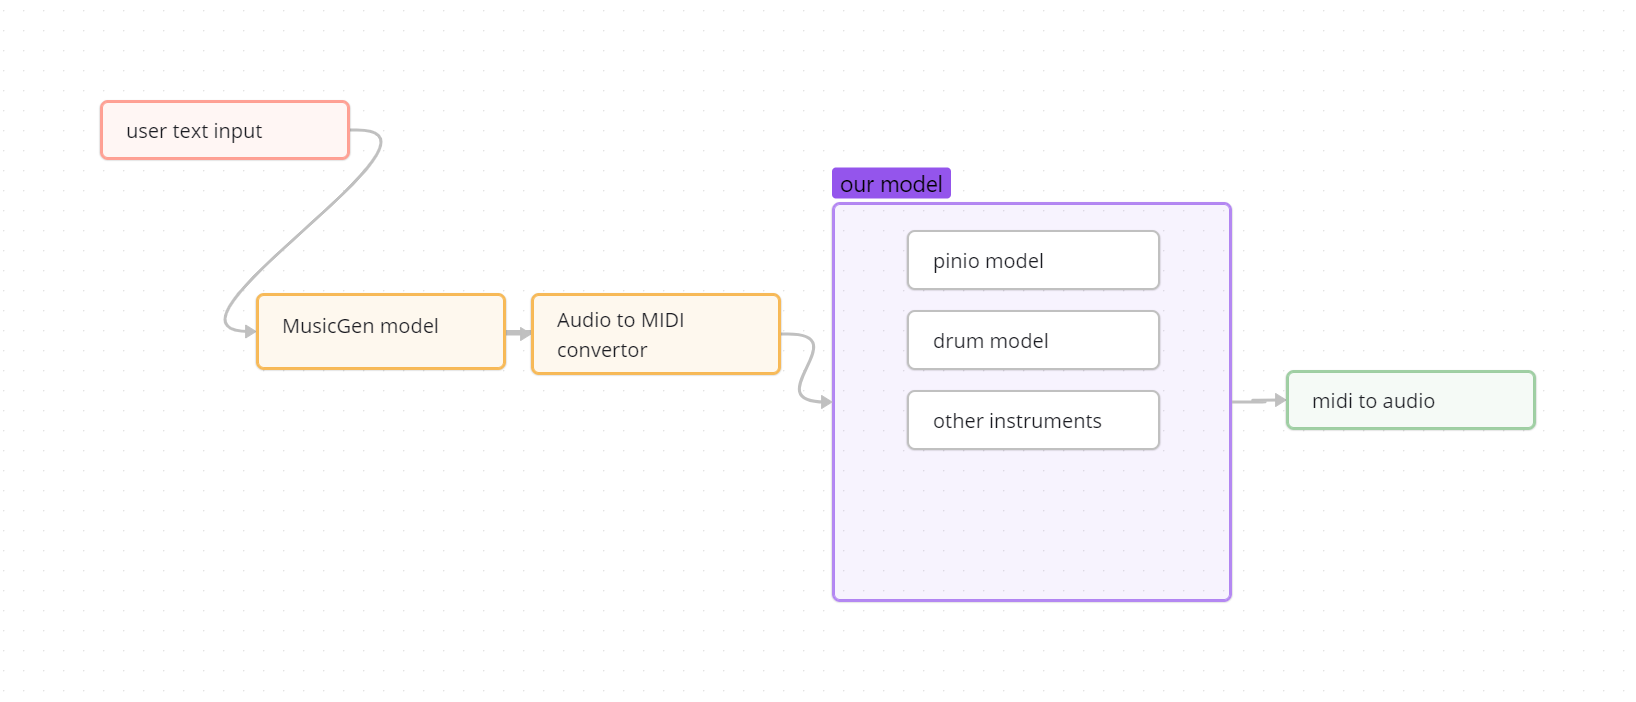
\includegraphics[scale=0.3]{Figures/pipe.png}
      \caption{ساختار  \lr{pipeline}
      }
      \label{Fig:Pipe}
\end{figure}


علاوه بر آموزش مدل‌ها، ما یک  \lr{pipeline} توسعه داده‌ایم که تجربه کاربری را بهبود می‌بخشد. این خط لوله همانطور که در \ref{Fig:Pipe} نشان داده شده است، ورودی متنی کاربر را دریافت کرده و آن را از طریق یک مدل تولید موسیقی \lr{(MusicGen)} \cite{copet2023simple} پردازش می‌کند. مدل \lr{MusicGen} یک فایل \lr{MIDI} بر اساس ورودی متنی کاربر ایجاد می‌کند. این فایل \lr{MIDI} تولید شده سپس از طریق مدل‌های آموزش دیده ما برای هر ساز عبور می‌کند. در نهایت، خروجی این مدل‌ها ترکیب شده و به عنوان ترکیب نهایی موسیقی ذخیره می‌شود.

با آموزش مدل‌های جداگانه برای هر ساز و ترکیب خروجی‌های آن‌ها، می‌توانیم به یک ترکیب موسیقیایی دقیق‌تر و پویا‌تر دست یابیم. این روش انعطاف‌پذیری و خلاقیت بیشتری در تولید موسیقی فراهم می‌کند، زیرا هر ساز می‌تواند به صورت جداگانه تنظیم شود و سپس در قطعه نهایی ادغام شود.

\section{دیتاسیت ها}
\subsection{مدل پیانو}

برای انجام آموزش مدل پیانو خود، ما از مجموعه داده گسترده‌ای به نام مجموعه داده \lr{MIDI} موسیقی ایرلندی \lr{IrishMMD} \cite{DBLP:conf/hcmir/WuLY023} استفاده کردیم. این مجموعه داده شامل 216,284 قطعه موسیقی ایرلندی به فرمت \lr{MIDI} است. این مجموعه داده به دو بخش تقسیم شده است: 99\% (214,122 قطعه) برای آموزش مدل و \%1 (2,162 قطعه) برای ارزیابی آن.

قطعات موسیقی این مجموعه داده از وب‌سایت‌های \lr{thesession.org} و \lr{abcnotation.com} جمع‌آوری شده‌اند. برای اطمینان از یکپارچگی داده‌ها، ممکن است برخی از قطعات موسیقی که به صورت متن بودند به فرمت \lr{MIDI} تبدیل شده باشند. همچنین، اطلاعات غیرموسیقی مانند عنوان و متن ترانه‌ها حذف شده است.
\subsection{مدل دارم}
\textbf{مجموعه داده گسترده \lr{EGMD} \cite{callender2020improving}}

برای تحقیق خود، ما از نسخه گسترده‌تری از مجموعه داده \lr{EGMD}
استفاده کردیم که به عنوان \textbf{مجموعه داده گسترده \lr{EGMD}}
شناخته می‌شود. \lr{GMD} یک مجموعه داده از اجراهای درام انسانی است که به صورت
\lr{MIDI} بر روی یک درام کیت الکترونیکی \lr{Roland TD-11} ضبط شده است.

\begin{table}[!ht]
      \centering
      \begin{tabular}{|l|l|l|l|}
            \hline
            بخش        & تعداد توالی‌های منحصربه‌فرد & تعداد کل توالی‌ها & مدت زمان (ساعت) \\ \hline
            آموزشی     & 819                       & 35,217           & 341.4           \\ \hline
            آزمایشی    & 123                       & 5,289            & 50.9            \\ \hline
            اعتبارسنجی & 117                       & 5,031            & 52.2            \\ \hline
            کل         & 1,059                     & 45,537           & 444.5           \\ \hline
      \end{tabular}
      \caption{خلاصه‌ای از مجموعه داده}
      \label{drumInfo}
\end{table}

ما تقسیم‌بندی‌های آموزشی، آزمایشی و اعتبارسنجی را که در \lr{GMD} وجود داشت، حفظ
کردیم. نکته مهم این است که از آنجایی که هر کیت برای هر توالی ضبط شده
است، تمام 43 کیت در بخش‌های آموزشی، آزمایشی و اعتبارسنجی وجود دارند. که به طور خلاصه در \ref{drumInfo} نشان داده شده است.


\section{تبدیل \lr{MIDI} به متن}

\section{رویکرد برای توکن‌سازی فایل‌های
  \lr{MIDI}}
\begin{itemize}
      \item {پیش‌پردازش}
            \begin{itemize}
                  \item
                        \textbf{فیلتر کردن}: حذف پیام‌های متا ناشناخته برای اطمینان از پردازش
                        فقط داده‌های \lr{MIDI} مرتبط.
                  \item
                        \textbf{ادغام ترک‌ها}: اگر فایل \lr{MIDI} شامل چندین ترک باشد، آن‌ها را به یک
                        ترک واحد ادغام کنید تا پردازش ساده‌تر شود.
            \end{itemize}

      \item {مدیریت وضعیت}

            \begin{itemize}

                  \item
                        \textbf{وضعیت کانال‌ها}: نگهداری دیکشنری‌هایی برای پیگیری وضعیت هر کانال
                        \lr{MIDI} شامل تغییرات برنامه، حجم، بیان، نوت‌های فعال و وضعیت پدال.
                  \item
                        \textbf{زمان‌بندی}: پیگیری زمان سپری شده بین رویدادهای \lr{MIDI} برای نمایش
                        دقیق زمان‌بندی در توالی توکن‌ها.
            \end{itemize}

      \item {بافر  توکن}

            \begin{itemize}

                  \item
                        \textbf{بافرینگ}: استفاده از یک بافر برای ذخیره موقت داده‌های توکن قبل
                        از تبدیل آن‌ها به توکن‌های رشته‌ای. این کار به مدیریت زمان‌بندی و توالی
                        توکن‌ها کمک می‌کند.
            \end{itemize}

      \item {پردازش رویدادها}

            \begin{itemize}

                  \item
                        \textbf{رویدادهای نوت}: پردازش رویدادهای \texttt{note\_on} و
                        \texttt{note\_off} برای شروع و توقف نوت‌ها، با در نظر گرفتن سرعت، حجم و
                        بیان.
                  \item
                        \textbf{تغییرات کنترل}: پردازش پیام‌های تغییر کنترل برای به‌روزرسانی
                        وضعیت کانال‌ها، مانند حجم، بیان و وضعیت پدال.
            \end{itemize}

      \item    {تولید توکن}

            \begin{itemize}

                  \item
                        \textbf{تبدیل توکن}: تبدیل داده‌های نوت بافر شده به توکن‌های رشته‌ای با
                        استفاده از فرمت‌های از پیش تعریف شده. این شامل نگاشت رویدادهای \lr{MIDI} به
                        نمایش‌های خاص توکن است.
                  \item
                        \textbf{توکن‌های زمان‌بندی}: تولید توکن‌هایی که زمان سپری شده بین
                        رویدادها را نمایش می‌دهند تا ساختار زمانی موسیقی حفظ شود.
            \end{itemize}

      \item{ساخت خروجی}

            \begin{itemize}

                  \item
                        \textbf{تقسیم قطعات}: تقسیم خروجی به قطعات بر اساس سکوت یا معیارهای
                        دیگر برای ایجاد بخش‌های قابل مدیریت از توکن‌ها.
                  \item
                        \textbf{نهایی‌سازی}: افزودن توکن‌های شروع و پایان به هر قطعه و ترکیب
                        لیست نهایی توالی‌های توکن.
            \end{itemize}

\end{itemize}

این رویکرد شامل پیش‌پردازش داده‌های \lr{MIDI}، مدیریت وضعیت کانال‌های \lr{MIDI}، بافر
کردن داده‌های توکن، پردازش رویدادهای مختلف \lr{MIDI}، تولید توکن‌ها و ساخت
خروجی نهایی است. این روش اطمینان می‌دهد که ساختار زمانی و موسیقیایی فایل
\lr{MIDI} به‌طور دقیق در توالی توکن‌ها نمایش داده می‌شود.

\begin{LTR}
      \begin{algorithm}
            \caption{توکن کردن فایل های \lr{MIDI}}
            \label{alg:token}
            \setmainfont{Times New Roman}
            \begin{algorithmic}[1]
                  \Function{mix\_volume}{velocity, volume, expression}
                  \State \Return $velocity \times \left(\frac{volume}{127.0}\right) \times \left(\frac{expression}{127.0}\right)$
                  \EndFunction

                  \Function{convert\_midi\_to\_str}{cfg, filter\_cfg, mid, augment=None}
                  \State Initialize state variables

                  \Function{flush\_token\_data\_buffer}{}
                  \State Convert token data buffer to token data
                  \State Append formatted tokens to output
                  \State Clear token data buffer
                  \EndFunction

                  \Function{consume\_note\_program\_data}{prog, chan, note, vel}
                  \If{token is valid}
                  \If{delta\_time\_ms $>$ threshold}
                  \State Check if any notes are held
                  \If{no notes are held}
                  \State Call \textproc{flush\_token\_data\_buffer}()
                  \State Append "<end>" to output
                  \State Reset output and state variables
                  \EndIf
                  \EndIf
                  \State Generate wait tokens and append to output
                  \State Reset delta\_time\_ms
                  \State Append token data to buffer
                  \State Set started\_flag to True
                  \EndIf
                  \EndFunction

                  \For{each msg in mid.tracks[0]}
                  \State Update delta\_time\_ms with msg.time

                  \Function{handle\_note\_off}{ch, prog, n}
                  \If{pedal is on}
                  \State Set pedal event
                  \Else
                  \State Call \textproc{consume\_note\_program\_data}(prog, ch, n, 0)
                  \State Remove note from channel\_notes
                  \EndIf
                  \EndFunction

                  \If{msg.type is "program\_change"}
                  \State Update channel\_program
                  \ElsIf{msg.type is "note\_on"}
                  \If{velocity is 0}
                  \State Call \textproc{handle\_note\_off}
                  \Else
                  \State Remove pedal event if exists
                  \State Call \textproc{consume\_note\_program\_data} with mixed volume
                  \State Add note to channel\_notes
                  \EndIf
                  \ElsIf{msg.type is "note\_off"}
                  \State Call \textproc{handle\_note\_off}
                  \ElsIf{msg.type is "control\_change"}
                  \State Update channel state based on control type
                  \Else
                  \State \textbf{pass}
                  \EndIf
                  \EndFor

                  \State Call \textproc{flush\_token\_data\_buffer}()
                  \State Append "<end>" to output
                  \State \Return output\_list
                  \EndFunction
            \end{algorithmic}
      \end{algorithm}
\end{LTR}

\begin{example}[]
      \centering
      \label{example:token}
      برای مثال \texttt{<start> 26:2 t8 26:0 26:2 t5 26:0 <end>} می تواند خروجی الگوریتم \ref{alg:token} باشد.
\end{example}

\subsection{توکن سازی}

در کار ما، از یک رویکرد ساده برای آماده‌سازی و آموزش مدل با استفاده از
کتابخانه \lr{Tokenizer} \cite{Moi_HuggingFace_s_Tokenizers_2023} استفاده کردیم. در اینجا توضیح دقیقی از این فرآیند
آورده شده است:

\subsubsection{توکن‌سازی سریع با کتابخانه \lr{Tokenizer}}

ما از کتابخانه \lr{Tokenizer} برای انجام توکن‌سازی سریع و کارآمد داده‌ها
استفاده کردیم. این کتابخانه برای پردازش مجموعه داده‌های بزرگ و تبدیل متن
خام به توکن‌ها به سرعت طراحی شده است. مزایای کلیدی استفاده از این
کتابخانه شامل موارد زیر است: - \textbf{سرعت}: کتابخانه \lr{Tokenizer} برای
عملکرد بهینه‌سازی شده است و به ما امکان می‌دهد حجم زیادی از داده‌ها را در
زمان کوتاهی پردازش کنیم. - \textbf{انعطاف‌پذیری}: این کتابخانه از
استراتژی‌های مختلف توکن‌سازی پشتیبانی می‌کند و به راحتی می‌توان آن را برای
نیازهای خاص پروژه سفارشی کرد.

\subsubsection{تبدیل به فرمت \lr{JSONL}}

پس از توکن‌سازی، داده‌های توکن‌شده را به فرمت \lr{JSON Lines (JSONL)} تبدیل
کردیم. این فرمت به خصوص برای پردازش مجموعه داده‌های بزرگ مناسب است زیرا:
- \textbf{پردازش خط به خط}: هر خط در یک فایل \lr{JSONL} نمایانگر یک شیء \lr{JSON}
جداگانه است که پردازش داده‌ها را خط به خط بدون نیاز به بارگذاری کل مجموعه
داده در حافظه آسان می‌کند. - \textbf{سادگی}: \lr{JSONL} به راحتی خوانده و
نوشته می‌شود و با بسیاری از ابزارهای پردازش داده‌ها به خوبی ادغام می‌شود.

\subsubsection{تبدیل به فرمت \lr{binidx} برای آموزش سریع}

برای بهینه‌سازی بیشتر فرآیند آموزش، داده‌های \lr{JSONL} را به فرمت \lr{binidx} تبدیل
کردیم. \lr{binidx} یک فرمت باینری است که چندین مزیت برای آموزش مدل‌های یادگیری
ماشین ارائه می‌دهد: - \textbf{کارایی}: فرمت‌های باینری به طور کلی فشرده‌تر
و سریع‌تر برای خواندن/نوشتن نسبت به فرمت‌های متنی هستند و سربار \lr{I/O} را در
طول آموزش کاهش می‌دهند. - \textbf{سازگاری}: فرمت \lr{binidx} با بسیاری از
چارچوب‌های یادگیری ماشین سازگار است و ادغام بدون مشکل در خط لوله آموزش ما
را تسهیل می‌کند. ما برای تبدیل فایل های \lr{JSONL} به فرمت \lr{binidx} از بخشی از کد های کتابخانه \lr{gpt-neox} \cite{gpt-neox-library} استفاده کردیم.

با استفاده از کتابخانه \lr{Tokenizer} برای توکن‌سازی سریع و تبدیل داده‌ها به
فرمت \lr{JSONL} و سپس به فرمت \lr{binidx}، ما به طور قابل توجهی کارایی فرآیندهای
آماده‌سازی داده و آموزش را بهبود بخشیدیم. این رویکرد به ما امکان داد تا
مجموعه داده‌های بزرگ را به طور مؤثر مدیریت کنیم و زمان کلی آموزش را تسریع
کنیم که منجر به توسعه کارآمدتر مدل شد.

\section{آموزش مدل}
\subsection{پارامترهای آموزش مدل}
در این بخش، پارامترهای مورد استفاده برای آموزش مدل توضیح داده شده‌اند:

ما از معماری \texttt{rwkv-6.0} \cite{peng2024eagle} استفاده کردیم. همچنین
امکان استفاده از مدل دارد. مدل ما شامل 20 لایه و
\lr{embedding} برابر با 512 است. \lr{Context Length} \footnote{\lr{Context Length} بی‌نهایت فقط در هنگام اجرای مدل معنا می  دهد.} مدل برابر با
512 است.
مقدار نرخ یادگیری اولیه و نهایی برابر با \num{6e-4}   و \num{6e-5} است.
\subsubsection{پیشرفت آموزش مدل}

\begin{figure}%
      \centering
      \subfloat[تغییر مقدار تابع خطا]{{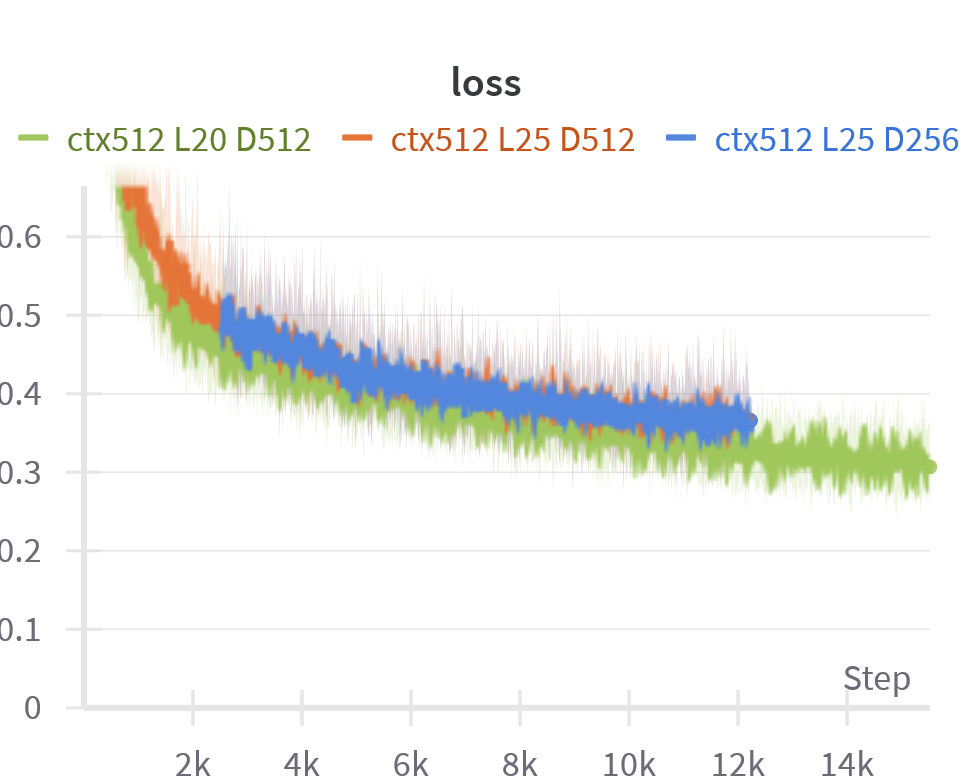
\includegraphics[width=8cm]{Figures/loss-pi.png} }}%
      \qquad
      \subfloat[تغییر نرخ یادگیری]{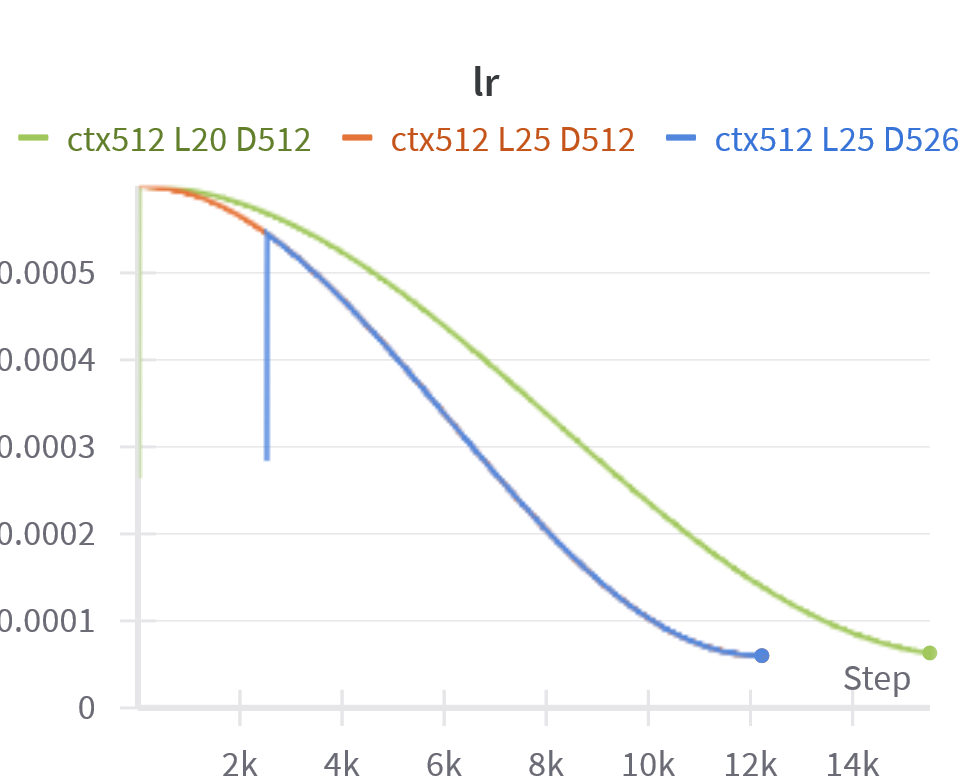
\includegraphics[width=8cm]{Figures/lr-pi.png} }%
      \caption{نمودار های پیشرفت یادگیری مدل پیانو}%
      \label{Fig:lrpi}%
\end{figure}

\begin{figure}%
      \centering
      \subfloat[تغییر مقدار تابع خطا]{{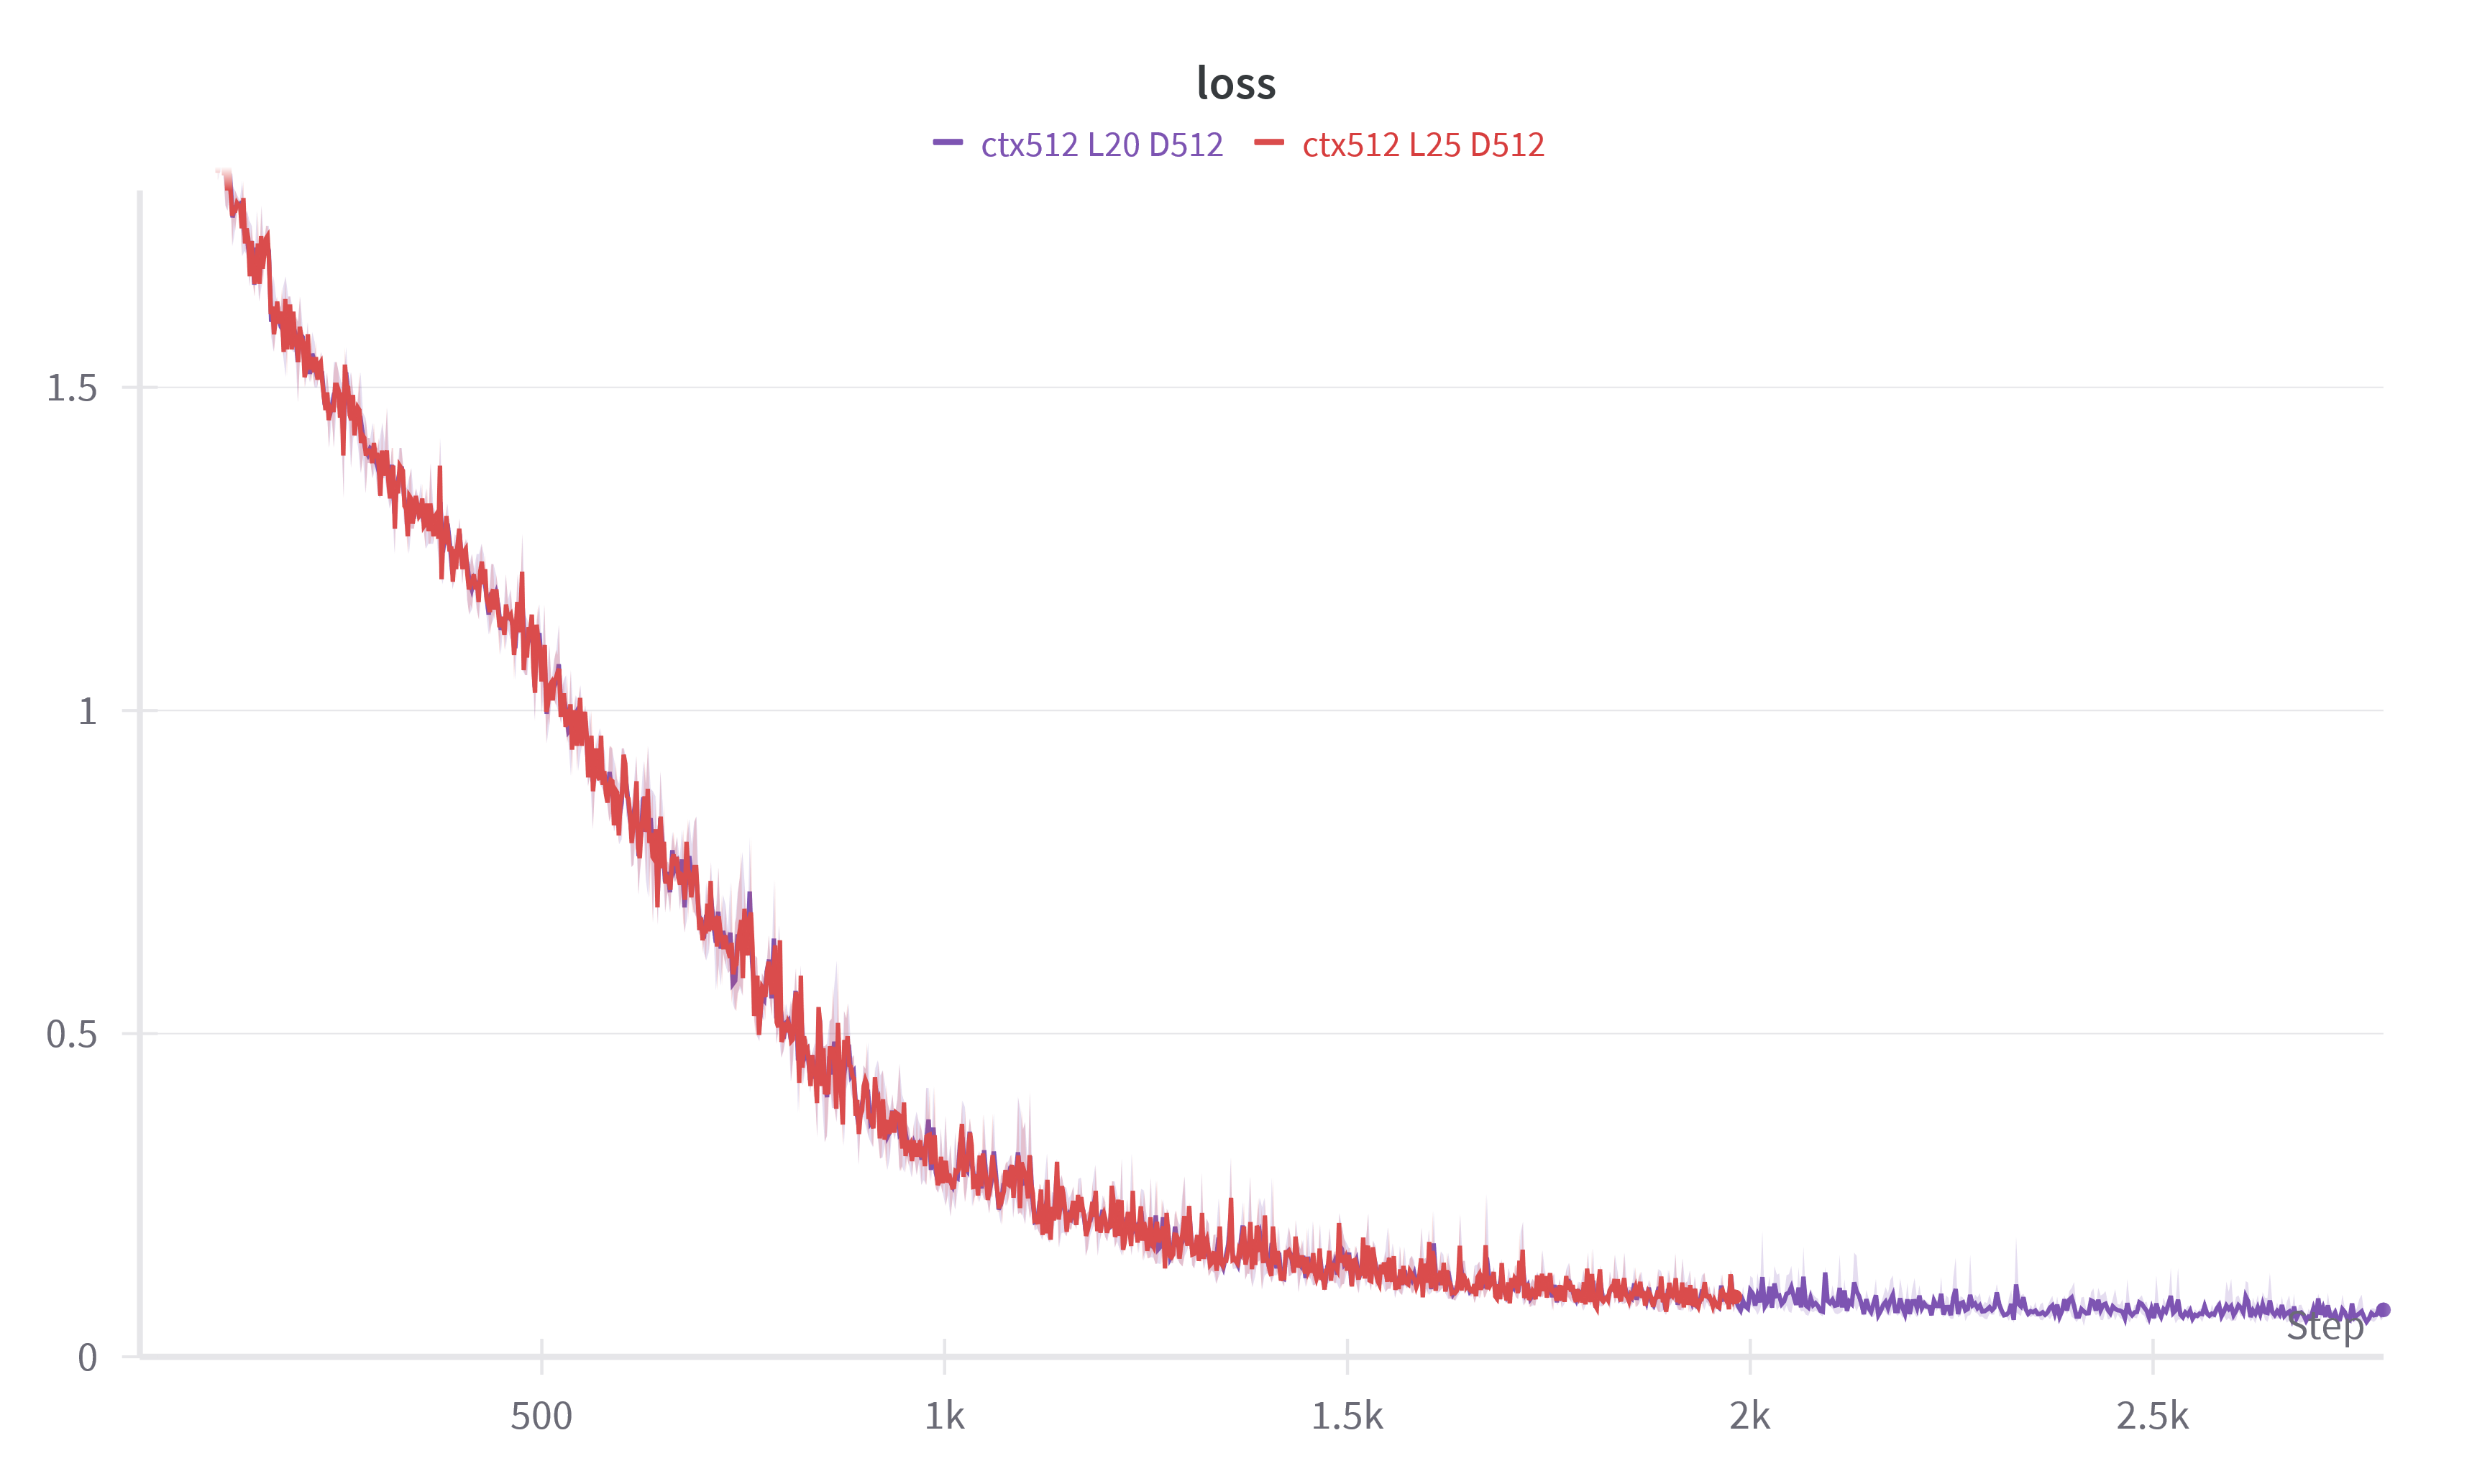
\includegraphics[width=8cm]{Figures/loss-dr.png} }}%
      \qquad
      \subfloat[تغییر نرخ یادگیری]{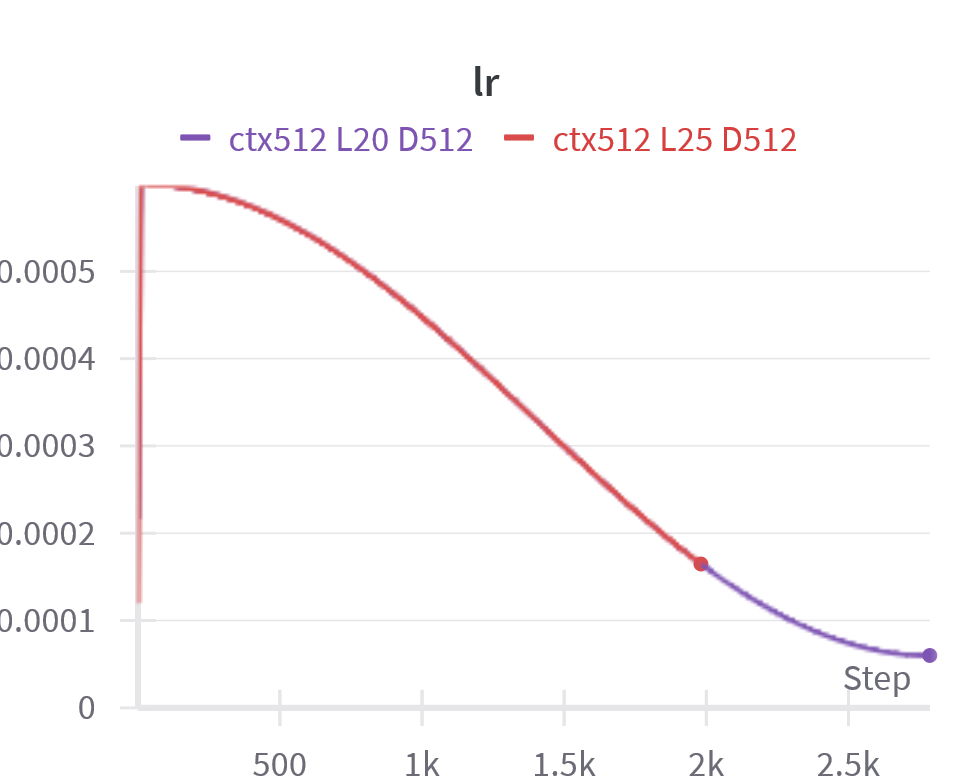
\includegraphics[width=8cm]{Figures/lr-dr.png} }%
      \caption{نمودار های پیشرفت یادگیری مدل درام}%
      \label{Fig:lrdr}%
\end{figure}